\documentclass[UTF8,10pt]{article}
\usepackage{ctex}%中文
\usepackage{amsmath}
\usepackage{graphicx}%插图
\usepackage{bookmark}
\hypersetup{hidelinks}
\usepackage{amstext}%数学环境中的文字
\usepackage{esint}%曲面积分符号
\usepackage{eucal}%特殊数学字体
\usepackage{geometry}
\usepackage{svg}
\geometry{a4paper,scale=0.8}


\begin{document}
\title{classical machenics}
\author{zhufeng}
\date{}
\maketitle
\thispagestyle{empty}%这一页的页码没有
\newpage%另起一页制作目录
\tableofcontents
\thispagestyle{empty}%这一页的页码没有
\newpage
\pagenumbering{arabic}%从正文开始计算页码
\setcounter{page}{1}
\section{基本原理概述}
\subsection{质点系的力学(machanics of a system of particals)}
外力与内力(external forces and internal forces),motion--运动,
So, the equation of motion for the ith is written as :
\begin{align*}
    \vec{F_{i}^{(e)}}+\sum_{j}\vec{F_{ji}}=\vec{p_i}'
\end{align*}
We say that internal force on the ith particals due to the jth particals.\\
Newton's 3rd law:
\begin{align*}
    \vec{F_{ij}}=-\vec{F_{ji}}
\end{align*}
Sum over the equation(1)
\begin{align*}
    \sum_{i}\vec{F_{i}^{(e)}}+\sum_{ji}\vec{F_{ji}}=\frac{d^2}{dt^2}\sum_i m_ir_i
\end{align*}
定义质心(the center of the mass)
\begin{align*}
    \vec{R} = \frac{\sum_im_ir_i}{\sum_i m_i}=\frac{\sum_im_i\vec{r_i}}{M}
    \Rightarrow M\frac{d^2R}{dt^2} =F^{(e)} = \sum_i F_i^{(e)}
\end{align*}
\subsection{质点系的动量守恒}
conservation theorem for linear momentum of a system of particals:
if the total external force is zero,the total linear momentum is conserved.\\
角动量(the total angular momentum)
\begin{align*}
    \vec{L}=\sum_i r_i\times \vec{p_i}
\end{align*}
prove:
\begin{align*}
    \frac{d\vec{L}}{dt}= & \sum_i \frac{d\vec{r_i}}{dt}\times \vec{p_i}+
    \sum_i \vec{r_i}\times\frac{d\vec{p_i}}{dt}                                  \\
    =                    & 0+\sum_i r_i\times F^{(e)}+\sum_{ij} r_i\times F_{ji}
\end{align*}
the strong law of action and reaction:
\[r_{ij}//F_{ij}\]
\newline
为了证明质心的角动量和质心系中质点的角动量之和相等,进行如下的推导:
\[\sum_{ij} r_i\times F_{ji} = \sum_i\vec{r_i}\times F_{ji}+\sum_j\vec{r_j}\times F{ij}\]

质心系下的角动量
\begin{align*}
    \vec{L}= & \sum_i\vec{L_i}                                                                                               \\
    =        & \sum_i \vec{r_i}\times m\vec{v_i}                                                                             \\
    =        & \sum_i (\vec{R}+\vec{r_i'})\times m(\vec{v_R}+\vec{v_i'})                                                     \\
    =        & \sum_i\vec{R}\times m\vec{v_R}+\sum_i\vec{R}\times m\vec{v_i'}+\sum_i\vec{r_i'}\times m\vec{v_R}
    +\sum_i\vec{r_i'}\times m\vec{v_i'}                                                                                      \\
    =        & \sum_i\vec{R}\times m\vec{v_R}+\sum_i\vec{R}\times \frac{\vec{dm r_i'}}{dt}+\sum_im\vec{r_i'}\times \vec{v_R}
    +\sum_im\vec{r_i'}\times \frac{d\vec{r_i'}}{dt}                                                                          \\
    =        & \sum_i \vec{R}\times m\vec{v_R}
\end{align*}
备注:
\begin{align*}
    R=                      & \frac{\sum m_{i} \vec{r}}{\sum m_{i}}        \\
    \sum m_{i} \vec{r}_{i}= & \sum m_{i}\left(\vec{R}-\vec{r}_{i}\right)=0
\end{align*}
\subsection{能量方程,质点系做功(the total kinetic energy)}
\begin{align}
    T=\frac{1}{2}\sum_i m_i (v_o+v_i')^2=\frac{1}{2}\sum_i m_i v_o^2+\frac{1}{2}
    \sum_i m_i v_i'^2+\frac{v}{2}\sum_i m_i \frac{dr_i'}{dt}
\end{align}
我们可以由前面的公式得到,equation(6)的第三项是0,于是我们得到了质点系得做功:
\begin{align}
    T=\frac{1}{2}\sum_i m_i (v_o+v_i')^2=\frac{1}{2}M v_o^2+\frac{1}{2}
    \sum_i m_i v_i'^2
\end{align}
现在我们开始推导出系统势能的总和:
\begin{align}
    \sum_i \int_{1}^{2 } F_i ds_i = \sum_i \int _{1}^{2} F^{(e)} ds_i +\sum
    _{i\neq j} F_{ji}ds_i
\end{align}
对于外力来说:
\begin{align}
    \sum_i \int _{1}^{2} F^{(e)} ds_i =-\sum_i \int_{1}^{2}  \nabla V_i d s_i=
    -\sum_iV_{i}|_{1}^{2}
\end{align}
对于内力来所说:
\begin{align}
    \vec{F}^{(in)}=-\nabla V_{ij}|\vec{r_i}-\vec{r_j}|= (\vec{r_i}-\vec{r_j})f(\text{标量函数})
\end{align}
然后可以推得:
\begin{align*}
    \int _{1}^{2} \vec{F}^{(in)} d\vec{s_i} & = -\sum_{i\neq j}\int_{1}^{2} \nabla_{ij} V_{ij}
    d\vec{r_{ij}}                                                                              \\
                                            & = -\frac{1}{2}\sum_{i\neq j} V_{ij}|_{1}^{2}
\end{align*}
将推导出来的势能函数代入到equation(8)当中,我们是可以系统的总的势能就是:
\begin{align*}
    V = -\sum_i V_i -\frac{1}{2}\sum_{i\neq j}V_{ij}
\end{align*}
\subsection{约束}
三类约束:
\begin{enumerate}
    \item 完全约束
    \item 非完全约束
    \item 含时问题与不含时间问题
\end{enumerate}
\section{拉格朗日方程}
以下推导均是在单演系统中:维基百科:In classical mechanics, a physical system is termed a monogenic system if the force acting on the system can be modelled in a particular, especially convenient mathematical form. The systems that are typically studied in physics are monogenic
\subsection{达朗贝尔原理与拉格朗日方程}
考虑在大部分情况下的约束力和运动方向垂直,利用达朗贝尔原理:我们的目标就是把相关的量全部化为其对应的广义坐标形式,然后代入达朗贝尔方程,然后就可以推导出拉格朗日方程
\begin{align*}
    \sum_i (\vec{F_i}-\dot{P_i})\delta r_i =0
\end{align*}

备注:在分析力学里,保持时间不变,虚位移是符合约束条件的无穷小位移。由于任何物理运动都需要经过时间的演进才会有实际的位移,所以称保持时间不变的位移为虚位移[1]。
动力学方程被化为了类似于静力学的方程,然后把速度换成含广义坐标表示的情况:
\begin{align*}
    \vec{v_i}=\frac{\vec{r_i}}{dt}=\frac{\partial \vec{r_i}}{\partial q}\frac{\partial q}{\partial t}+\frac{\partial \vec{r_i}}{\partial t}
\end{align*}
虚位移化成广义坐标的形式:
\[\delta \vec{r_i}=\frac{\partial \vec{r_i}}{\partial q}\partial q\]
虚功:$W=\sum_i \vec{F_i}\delta \vec{r_i}=\sum_i \vec{F_i}\frac{\partial\vec{r_i}}{\partial q} \partial q=\sum_i Q_j \delta q_j$,其中$Q_j$是广义力,现在对后面的能量做变换:
\begin{align*}
    \frac{d mv_i}{dt}=m\ddot{\vec{r}}_i\delta \vec{r_i}=m\ddot{\vec{r}}_i\frac{\partial\vec{r}_i}{\partial q}\delta q
\end{align*}
现在我们要将其化为仅含速度和位置的方程,因为我们最后是要将坐标和能量联系起来的方程
$$\sum_{i} m \ddot{\vec{r}}_{i} \frac{\partial \vec{r}_{i}}{\partial q_{j}}=\sum_{i} \left[ m \frac{d}{d t}\left(\dot{\vec{r}}_{i} \frac{\partial \vec{r}_{i}}{\partial q_{j}}\right)-m \dot{r}_{i} \frac{d}{d t}\left(\frac{\partial \vec{r}_{i}}{\partial q_{j}}\right)\right]$$
得到:
$$-\sum_{i}\left(\frac{d}{d t} \frac{\partial\left(\frac{1}{2} m \vec{v}_{i}^{2}\right)}{\partial \dot{q}_{j}}-\frac{\partial\left(\frac{1}{2} m \vec{v}_{i}^{2}\right)}{\partial q_{j}}-Q_{j}\right) \delta q_{j}=0$$
最后根据:$-\nabla V=F,Q_j=\sum_i F_i\frac{\partial \vec{r}_i}{\partial q_j}$,得到:
$$\frac{d}{d t}\left(\frac{\partial(T-V)}{\partial \dot{q}_{j}}\right)-\frac{\partial(T-V)}{\partial q_{j}}=0$$
既可以得到拉格朗日方程:
\begin{align*}
    \frac{d}{dt}\frac{\partial L}{\partial \dot{q}_j}-
    \frac{\partial L}{\partial q_j}=0
\end{align*}
\subsection{变分法导出拉格朗日方程}
\begin{align*}
    \delta t= \int _{x_1}^{x_2} f(x,y,y') dx =0
\end{align*}
泛函维基百科:泛函(functional)指以函数构成的向量空间为定义域,实数为值域为的“函数”,即某一个依赖于其它一个或者几个函数确定其值的量,往往被称为“函数的函数”。在泛函分析中,泛函也用来指一个从任意向量空间到标量域的映射。泛函中的一类特例线性泛函引发了对对偶空间的研究。泛函的应用可以追溯到变分法,其中通常需要寻找一个函数用来最小化某个特定泛函。在物理学上,寻找某个能量泛函的最小系统状态是泛函的一个重要应用。
\\引入无穷小量参数$\alpha$,并且使得$\eta(x_1)=\eta(x_2)$使得只与路径积分有关,此时的$f(x,\alpha)=f(x)+\alpha\eta(x)$
利用变分法基本引理,详见维基百科
\subsection{哈密顿原理推导出拉格朗日方程}
\begin{align*}
    \mathcal{S}=\int _{t_1}^{t_2} L(q,\dot{q}(t),t) dt
\end{align*}
$\mathcal{S}$被称为作用量
先使用文字描述以下哈密顿原理:对于正确的路径的作用量具有平稳值,数学描述:
\[\frac{\delta \mathcal{S}}{\delta q(t)}=0\]
Hamilton's principle requires that this first-order change $\displaystyle \delta \mathcal {S}$ is zero,我们引入一个无穷小量$\epsilon$,则:
\begin{align*}
    \delta \mathcal{S}=\int_{t_1}^{t_2} (L(q+\epsilon,\dot{q}+\dot{\epsilon},t)-L(q,\dot{q},t))dt=\int_{t_1}^{t_2}(\epsilon \frac{\partial L}{\partial \dot{q}}+\dot{\epsilon}\frac{\partial L}{\partial q})dt
\end{align*}
其中利用了导数的定义,其中:$\epsilon(t_1)=\epsilon(t_2)=0$,然后对第二项利用分部积分:
\begin{align*}
    \int_{t_1}^{t_2}{\epsilon \frac{\partial L}{\partial q}}dt+\int_{t_1}^{t_2}{\frac{\partial L}{\partial \dot{q}}}d\left( \epsilon \right)
    = & \int_{t_1}^{t_2}{\epsilon \frac{\partial L}{\partial q}}dt+\epsilon\frac{\partial L}{\partial \dot{q}}|_{t_1}^{t_2}
    -\int_{t_1}^{t_2}\epsilon \frac{d}{dt}(\frac{\partial L}{\partial \dot{q}})                                                                                                  \\
    = & \epsilon\frac{\partial L}{\partial \dot{q}}\vert_{t_1}^{t_2}+\int_{t_1}^{t_2}\epsilon(\frac{\partial L}{\partial q}-\frac{d}{dt}(\frac{\partial L}{\partial \dot{q}}))=0
\end{align*}
式中第一项为0,因此我们可以得出拉格朗日方程。
\section{两体有心力问题(two body central force problem)}
\subsection{等效为一维问题}
两个质点所受的保守有心力且无其他外力,两个质点的质量$m_1,m_2$,其位置矢量$\vec{r_1},\vec{r_2}$
双星系统相互之间的引力。
\[F=G\frac{m_1m_2}{(\vec{r_1}-\vec{r_2})^2}\Rightarrow V=-G\frac{m_1m_2}{|\vec{r_1}-\vec{r_2}}|\]
上述系统只依赖于质点的相对位置$r=\vec{r_1}-\vec{r_2}$,中心力场与r的方向无关,只与r的大小有关
\\简化为单体问题:
% \begin{center}
%     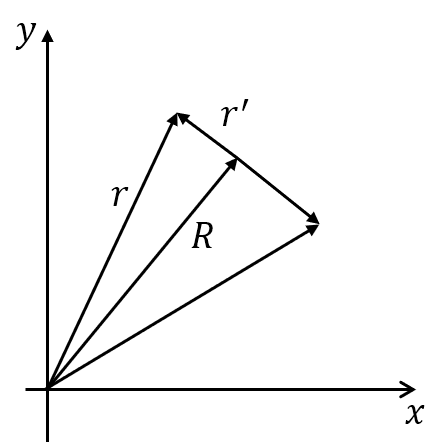
\includegraphics[scale=0.6]{img/图片1.png}
% \end{center}
质心矢径:$$R=\frac{m_1\vec{r_1}+m_2\vec{r_2}}{m_1+m_2}$$
相对矢径(relative position vector)
\begin{align*}
    \vec{r}=   & \vec{r_1}-\vec{r_2}                \\
    \vec{r_1}= & \vec{R}+\frac{m_2}{m_1+m_2}\vec{r}
\end{align*}
\[r'=r_1-R=r_1-\frac{m_1\vec{r_1}+m_2\vec{r_2}}{m_1+m_2}=\frac{m_2 r}{m_1+m_2}\]
$$
    T=\frac{1}{2}m({\dot{\vec{r}}_1}^2+{\dot{\vec{r}}_2}^2)=\frac{1}{2}\left( M\dot{\vec{R}}^2+\frac{m_1m_2}{M}\dot{\vec{r}}^2 \right) ,M=m_1+m_2
$$
引入约化质量(reduced mass)$u=\frac{m_1m_2}{m_1+m_2}$
一个循环坐标对应一个守恒量,又拉格朗日量:
$$
    L=T-V=\frac{1}{2}M\dot{\vec{R}}^2+\frac{1}{2}u\dot{\vec{r}}^2-V\left( r \right)
$$
L不显含R,R是循环坐标,因此对R的广义动量守恒,既$m\dot{\vec{R}}=constant$,质心是静止的或者均速运动的
,此时的拉格朗日方程就变成了
$$
    L=T-V=\frac{1}{2}u\dot{\vec{r}}^2-V\left( r \right)
$$
到现在已经变成了一个单体问题,只有三个自由度。
\subsection{运动方程和初次积分}
现在讨论保守的有心力场问题,根据前面的我们只需要考虑相对于力心得问题就可以了
对于平面极坐标形式下得拉氏函数:
$$
    L=T-V=\frac{1}{2}m\left( \dot{r}^2+r^2\dot{\theta}^2 \right) -V\left( r \right)
$$
其中$\theta$是循环坐标,因此其对应得正则动量(广义动量是守恒的),$mr^2\dot{\theta}=l(\text{l是角动量常数})$
掠面速度:$\frac{dA}{dt}=\frac{1}{2}r^2\dot{\theta}=C$,证明开普勒行星第二定律
掠面速度守恒是有心力运动的普偏性质,不局限于平方反比定律。\\
还有一个关于r的拉个朗日方程:
\begin{equation*}
    \frac{d}{d t}(m \dot{r})-m r \dot{\theta}^{2}+\frac{\partial V}{\partial r}=0
\end{equation*}
\begin{equation*}
    m \ddot{r}-m r \dot{\theta}^{2}=f(r)
\end{equation*}
$$
    m \ddot{r}-\frac{l^{2}}{m r^{3}}=f(r)
$$
还有一个守恒方程:
$$
    E=\frac{1}{2} m\left(\dot{r}^{2}+r^{2} \dot{\theta}^{2}\right)+V(r)
$$
我们现在整合一个上面得到的3个方程:
$$
    \begin{cases}
        mr^2\dot{\theta}=l(\text{l是角动量常数)}                       \\
        m \ddot{r}-\frac{l^{2}}{m r^{3}}=f(r)                          \\
        E=\frac{1}{2}m\left( \dot{r}^2+r^2\dot{\theta}^2 \right) +V(r) \\
    \end{cases}
$$
然后我们可以得到两个微分方程,然后求解,可以得到$r,\theta$关于t的函数
$$
    \dot{r}=\sqrt{\frac{2}{m}\left(E-V-\frac{l^{2}}{2 m r^{2}}\right)}
$$
这里我们来分析一下E取各种值时,质点的运动状态。
\begin{align*}
    E=\frac{1}{2}m\dot{r}^2+V_{eff}
\end{align*}
假设$V(r)=-\frac{k}{r}$,且$V_{eff}=\frac{1}{2}mr^2\dot{\theta}^2+-\frac{k}{r}$
,$V_{eff}$为有效势能。我们结合图像可以得到:

% \begin{center}
%     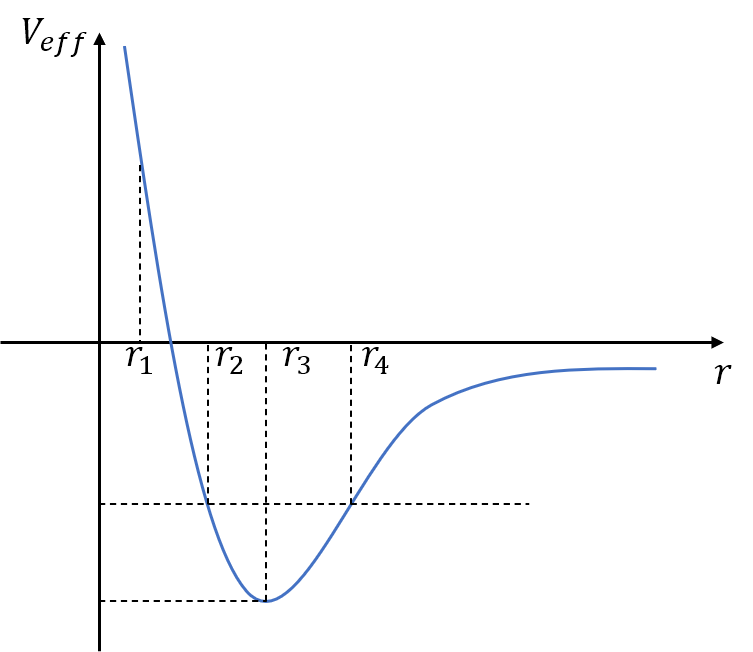
\includegraphics[scale=0.6]{img/有效势能.png}
% \end{center}
\begin{description}
    \item[A.] $E\geq 0$,存在一个$V_{eff}$的值恰好使得在动能项等于0的情况下,上面的式子的等号成立,所以$r\geq r_1$.
    \item[B.] $E\leq 0$,此时的速度为虚数,并且$V_{eff}$也是小于0的状态,$r_2\leq r\leq r_4$
    \item[C.] $E=E_{min}$,此时的$V_{eff}=0,f(r)=\frac{-l^2}{mr^3}$
\end{description}
\subsection{维里定理}
可用于有心力场的统计力学,量子力学,力学量的时间平均值的定理,定义:
$$
    G=\sum_i{\vec{p}_i\cdot \vec{r}_i, \frac{dG}{dt}=\sum_i{\left( \dot{\vec{p}}_i\cdot \vec{r}_i+\vec{p}_i\cdot \dot{\vec{r}}_i \right)}}
$$
其中第二项为2T,第一项$\vec{F_i}\cdot \vec{r_i}$,因此:
$$
    \frac{dG}{dt}=2T+\sum_i{\vec{F}_i\vec{r}_i}
$$
考虑时间间隔$\tau$内的平均值:
\begin{align*}
    \frac{1}{\tau}\int_{0}^{\tau} dt & = 2\overline{T}+\overline{\sum_i \vec{F_i}\vec{r_i}} \\
                                     & =\frac{1}{\tau}[G(\tau)-G(0)]
\end{align*}
1、若为周期运动,$\tau$为周期时间则等式右端为0,\\
2、一般的,$\tau\rightarrow \infty$,等式右端趋近于0.\\
此时的$2\overline{T}=-\overline{\sum_i \vec{F_i}\vec{r_i}}$,称为维里定理,等式右端叫做维里,克劳修斯引入。
\\考虑到:$\vec{F_i}=-\nabla_i V$,且V是r的齐次函数,$V=\alpha r^{n+1}$
,代入得到:
\begin{align*}
    \overline{T}=\frac{1+n}{2}\overline{V}
\end{align*}
例如对于符合平方反比的力n=-2,则$\overline{T}=-\frac{1}{2}\overline{V}$,对于谐振子n=1,则$\overline{T}=\overline{V}$。
\subsection{开普勒问题}
我们现在继续分析之前的微分方程,这里我们假设的$V(r)=-\frac{1}{k}$:
\begin{align*}
    \frac{dr}{dt}=   & \sqrt{\frac{2}{m}(E-V(r))-\frac{l^2}{2mr^2}},
    \frac{d\theta}{dt}=\frac{l^2}{mr^2}                                             \\
    \theta-\theta_0= & \int_{r_0}^r dr \frac{l/r^2}{\sqrt{2m(E-V)-\frac{l^2}{r^2}}}
\end{align*}
这里,$V(r)=-\frac{k}{r},u=\frac{1}{r},du=-\frac{dr}{r^2}$,则我们把积分变成:
\begin{align*}
    \theta-\theta_0= & \int_{r_0}^r dr \frac{l/r^2}{\sqrt{2m(E-V)-\frac{l^2}{r^2}}}        \\
    =                & -\int_{u_0}^u\frac{du}{\sqrt{\frac{2mE}{l^2}+\frac{2mku}{l^2}-u^2}}
\end{align*}
由积分公式:
\begin{align*}
    \int\frac{dx}{\sqrt{\alpha+\beta x+\gamma x^2}}=\frac{1}{-r}\arccos[-(\beta+2\gamma x)/\sqrt{q}] \\
    \text{其中:}\alpha=\frac{2mE}{l^2}, \beta=\frac{2mk}{L^2},r=-1
\end{align*}
\begin{align*}
    \theta = -\arccos(\frac{l^2/mkr-1}{\sqrt{1+2El^2/mk^2}})
\end{align*}
引入:$p=l^2/mk,\epsilon=\sqrt{1+\frac{2El^2}{mk^2}}$,因此我们可以得到运动的轨道方程:
\begin{align*}
    r=\frac{p}{1+\epsilon \cos \theta}(\text{近日点})
\end{align*}
圆锥曲线极坐标参数方程,$\epsilon$偏心率,轨道性质与$\epsilon$有关,我们可以得到以下关系:
\begin{description}
    \item[1.] $\epsilon > 1,E>0$双曲线
    \item[2.] $\epsilon=0,E=0$ 抛物线
    \item[3.] $\epsilon<0,E<0$ 椭圆
    \item[4.] $\epsilon=0,E=-\frac{mk^2}{2}$ 圆
\end{description}
对于椭圆轨道:
% \begin{center}
%     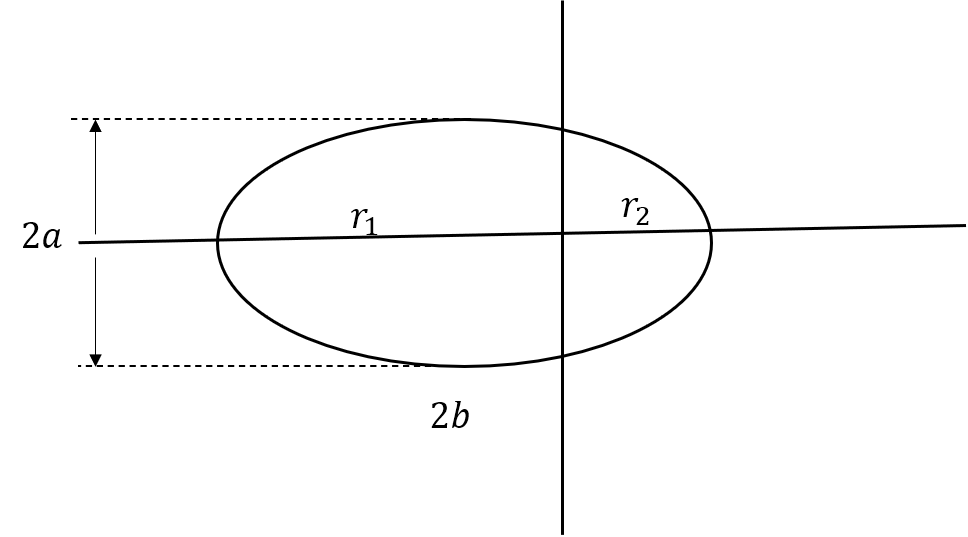
\includegraphics[scale=0.6]{img/椭圆1.png}
% \end{center}
\begin{align*}
    2a=r_1+r_2=\frac{p}{1+\epsilon}+\frac{p}{1-\epsilon} \\
    a=\frac{p}{(1-\epsilon)(1+\epsilon)}=\frac{k}{|E|}   \\
    b=\frac{p}{\sqrt{1-\epsilon^2}}=\frac{l}{2mE}
\end{align*}
椭圆面积,$A=\pi ab,\frac{dA}{dt}=\frac{l}{2m}$,解这个微分方程,$T=2\pi a^{\frac{3}{2}}\sqrt{m/k}\Rightarrow T^2\sim a^3$,开普勒第三定律
\section{耦合谐振子(small ocallations)}
偏离平衡位置较小:耦合谐振子,应用:声学,分子谱,耦合电路
\subsection{一维简谐振动}
\begin{gather*}
    T=\frac{1}{2}mv^2,V=\frac{1}{2}kx^2\\
    L=\frac{1}{2}mv^2-\frac{1}{2}kx^2\\
    \frac{d}{dt}(\frac{\partial L}{\partial\dot{x}})-\frac{\partial L}{\partial x}=0\\
    m\ddot{x}+kx=0
\end{gather*}
解的形式:$x(t)=A\cos( \omega t+\phi)$
若拉格朗日量不显含时间t,则E守恒,$\frac{\partial (L+V)}{\partial t}=0$
对于V在平衡位置取极值:$Q_i=-(\frac{\partial V}{\partial q_i})=0$,V在平衡位置时
取极值,偏离很小位置:$q_i=q_{i_0}+n_j$
\subsection{推广到多自由度体系的小振动}
n个自由度对应着n个广义坐标:$q_1\cdots q_n$,变换方程不依赖于时间:$r_i=r_i(q_1\cdots q_n)
$势能V在极值点附近进行泰勒展开:
\begin{equation*}
    V(q_i\cdots q_n)=\cdots+(\frac{\partial V}{\partial q_i})_0\eta_i
    +\frac{1}{2!}(\frac{\partial^2 V}{\partial q_i \partial q_j})\eta_i\eta_j
\end{equation*}
上式用到了爱因斯坦求和约定,满足平衡条件时,线性项为0,则:
\[V=\frac{1}{2}(\frac{\partial^2 V}{\partial q_i \partial q_j })\eta_i\eta_j
    =\frac{1}{2}\partial_{ij}V \eta_i\eta_j\]
将动能化成由广义坐标表示的形式:
\[T=\frac{1}{2}m_i v_i^2=\frac{1}{2}(\frac{\partial r_i}{\partial q_i}\dot{q_i}+\frac{\partial r_i}{\partial t})\]
变换方程与时间无关:
\begin{align*}
    T= & \frac{1}{2}m_{jk}\dot{q_i}\dot{q_j} \\=&\frac{1}{2}m_i\frac{\partial r_i}{\partial q_j}\frac{\partial r_i}{\partial q_i}\dot{q_i}\dot{q_j}
\end{align*}
在平衡点进行泰勒展开:
\begin{gather*}
    m_{ij}(q_i\cdots q_n)=m_{ij}(q_{i0}\cdots q_{n0})+\frac{\partial m_{ij}}{\partial q_k}\eta_k
\end{gather*}
其中线性项不是0,又$(x-q_{i0})'=v$则动能改写为:
\begin{gather*}
    T=\frac{1}{2}m_{ij}(q_{i0}\cdots q_{n0})\dot{\eta_i}\dot{\eta _j}=\frac{1}{2}T_{ij}\dot{\eta_i}\dot{\eta_j}
\end{gather*}
得到lagrangian:
\[L=T-V=\frac{1}{2}(T_{ij})\dot{\eta_i}\dot{\eta _j}-V_{ij}\eta_i\eta_j\]
$\eta$为新的广义坐标,对于quadrat form,由E-L方程得到耦合谐振子方程:
\[T_{ij}\ddot{\eta_j}+V_{ij}\eta_j=0\]
其中$T_{ij}=T_{ji},V_{ij}=V{ji}$,这里的T和V可以看出张量,也就是矩阵分量,二阶张量的
表达形式
\subsection{本征值方程(characteristtic equation)}
通解:$\eta =Ca_ie_{\pm i\omega t}$,e指数项系数可以是复数,广义坐标$\eta_i$的复振幅
通解代入耦合谐振子方程,得到:
\begin{align*}
    (V_{ij}-\omega^2T_{ij})a_j=         & 0 \\
    (\bar{V}-\omega ^2 \bar{T})\vec{a}= & 0
\end{align*}
要求系数行列式$det(\bar{V}-\omega^2\bar{T})=0$
\subsection{线性三原子分子的自由振动}
% \begin{center}
%     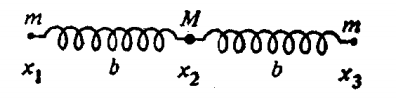
\includegraphics[scale=0.4]{img/QQ截图20210505144219.png}
% \end{center}
解:设平衡位置时的弹簧的长度为b,每个质点的初始位置是$x_{01},x_{02},x_{03}$.
\\对于系统的势能:$$V=\frac{1}{2}k(x_2-x_1-b)^2+\frac{1}{2}k(x_3-x_2-b)^2$$
又$x_{02}-x_{01}=b=x_{03}-x_{02},\eta_i=x_i-x_{0i}$
\begin{align*}
    V & =\frac{1}{2}k(\eta_2-\eta_1)^2+\frac{1}{2}k(\eta_3-\eta_2)^2                                                                            \\
      & =\frac{1}{2}k\left( {\eta _1}^2+{\eta _2}^2-2\eta _1\eta _2 \right) +\frac{1}{2}k\left( {\eta _3}^2+{\eta _2}^2-2\eta _2\eta _3 \right) \\
      & =\frac{1}{2}k\left( {\eta _1}^2+{\eta _3}^2+2{\eta _2}^2-2\eta _1\eta _2-2\eta _2\eta _3 \right)
\end{align*}
对应的矩阵形式:
$$
    \left( \begin{matrix}
            \eta _1 & \eta _2 & \eta _3 \\
        \end{matrix} \right) \left( \begin{matrix}
            k  & -k & 0  \\
            -k & 2k & -k \\
            0  & -k & k  \\
        \end{matrix} \right) \left( \begin{array}{c}
            \eta _1 \\
            \eta _2 \\
            \eta _3 \\
        \end{array} \right)
$$
对于动能项:
$$
    T=\frac{1}{2}{m\dot{\eta}_1}^2+\frac{1}{2}{M\dot{\eta}_2}^2+\frac{1}{2}{m\dot{\eta}_3}^2
$$
写成矩阵形式
$$
    \left( \begin{matrix}
            \eta _1 & \eta _2 & \eta _3 \\
        \end{matrix} \right) \left( \begin{matrix}
            m & 0 & 0 \\
            0 & M & 0 \\
            0 & 0 & m \\
        \end{matrix} \right) \left( \begin{array}{c}
            \eta _1 \\
            \eta _2 \\
            \eta _3 \\
        \end{array} \right)
$$
代入本征值方程:
$(\bar{V}-\omega ^2 \bar{T})\vec{a}=0$
$$
    \left[ \left( \begin{matrix}
            k  & -k & 0  \\
            -k & 2k & -k \\
            0  & -k & k  \\
        \end{matrix} \right) -\omega ^2\left( \begin{matrix}
            m & 0 & 0 \\
            0 & M & 0 \\
            0 & 0 & m \\
        \end{matrix} \right) \right] \vec{a}=0
$$
$$
    \left( \begin{matrix}
            k-\omega ^2m & -k            & 0            \\
            -k           & 2k-\omega ^2M & -k           \\
            0            & -k            & k-\omega ^2m \\
        \end{matrix} \right) =\omega ^2\left( k-\omega ^2m \right) \left( k(M+2m)-\omega^2Mm \right) =0
    \\
$$
因此解为:$$\omega_1=0,\omega_2=\sqrt{\frac{k}{m}},\omega_2=\sqrt{\frac{k(M+2m)}{Mm}}$$
对于这三个$\omega$代入到原方程,可以算出a向量分量之间的关系,对应三个模式。\\
$\omega=0$时:
\begin{equation*}
    \begin{array}{l}
        \left(\begin{array}{ccc}
                      k  & -k  & 0  \\
                      -k & 2 k & -k \\
                      0  & -k  & k
                  \end{array}\right)\left(\begin{array}{l}
                                              a_{1} \\
                                              a_{2} \\
                                              a_{3}
                                          \end{array}\right)=0 \\
        \left\{\begin{array}{l}
                   a_{1} k-k a_{2}=0 \Rightarrow a_{1}=a_{2} \\
                   -k a_{1}+2 k a_{2}-k a_{3}=0              \\
                   -a_{2} k+k a_{3}=0 \Rightarrow a_{2}=a_{3}
               \end{array}\right.
    \end{array}
\end{equation*}
对应的模式:$$\left(1,1,1\right)a_1$$
$\omega=\sqrt{\frac{k}{m}}$时:
$$\left(1,0,-1\right)a_1$$
$\omega=\sqrt{\dfrac{k(M+2m)}{Mm}}$时:
$$
    \left( 1,1-\frac{M+2m}{M},1\right)a_1
$$

\section{刚体运动学}
类似于在笛卡尔坐标当中,一个点的坐标可以有三个距离确定,这个点到x轴的距离,到y,z轴的距离,在描述刚体时,应该说也是类似的,刚体可以用六个自由度来描述,其中只需要确定三个点的位置,剩下的点的位置就
可以确定了,刚体上任意一点到这三个点的距离。
\subsection{正交变换}
行向量和列向量相互正交的单位矩阵满足正交矩阵,相互正交的条件使得其转置矩阵
和逆矩阵是相等的。
\begin{align*}
    Q^T Q=I\Rightarrow Q^{-1}Q =I
\end{align*}
作为线性映射,正交矩阵保持距离不变,是一个保距映射,具体例子有:旋转,镜面反射
,对称。

现在讨论对于低维空间中正交矩阵的性质,
对于矩阵:
\begin{align*}
    \left[
        \begin{matrix}
            p & t \\
            q & u \\
        \end{matrix}
        \right]
\end{align*}
对于横向量满足正交归一性,正交性:
\begin{align*}
    pq+tu=0
\end{align*}
归一性:
\begin{align*}
    \left\{
    \begin{array}{c}
        p^2+t^2=1 \\
        q^2+u^2=1
    \end{array}
    \right.
\end{align*}
记住我们以后遇到旋转,对称和镜面反射需要联想到正交矩阵。
\subsection{欧拉角}
欧拉角的形成分为三步,先绕z轴旋转$\varphi$角,绕$x'$轴旋转$\theta$角,绕$z''$角
旋转$\phi$角。
\begin{gather*}
    x=\left( \begin{array}{c}
        \xi   \\
        \eta  \\
        \zeta \\
    \end{array} \right)
    \quad
    x''=\left( \begin{array}{c}
        \xi'   \\
        \eta'  \\
        \zeta' \\
    \end{array} \right)
    \quad
    x'''=\left( \begin{array}{c}
        \xi'''   \\
        \eta'''  \\
        \zeta''' \\
    \end{array} \right)
\end{gather*}
之前我们引入了转动$\phi$角的矩阵:
\begin{gather*}
    \vec{x'}=D \vec{x}\\
    \vec{x''}=C \vec{x'} \\
    \vec{x'''}=B \vec{x''}
\end{gather*}
三个矩阵算子分别是:
$$
    D=\left[ \begin{matrix}
            \cos \phi  & \sin \phi & 0 \\
            -\sin \phi & \cos \phi & 0 \\
            0          & 0         & 1 \\
        \end{matrix} \right] \,\, C=\left[ \begin{matrix}
            1 & 0            & 0           \\
            0 & \cos \theta  & \sin \theta \\
            0 & -\sin \theta & \cos \theta \\
        \end{matrix} \right] \,\,B=\left[ \begin{matrix}
            \cos \phi  & \sin \phi & 0 \\
            -\sin \phi & \cos \phi & 0 \\
            0          & 0         & 1 \\
        \end{matrix} \right]
$$
\subsection{无限小转动}
对于有限小的转动和转动的顺序是有关的,但是对于无限小的转动,与顺序是无关的,
设无线小的转动是可以这样变换的:
\begin{align*}
    x_{i}'=x_i+\varepsilon_{ij}x_j=(\delta_{ij}+\varepsilon_{ij})x_{ij}
\end{align*}
$\delta_{ij}$是单位矩阵的矩阵元,则上面的变换可以是:
\begin{align*}
    x=(I+\varepsilon)x
\end{align*}
现在考虑到两次无线小的转动
\begin{align*}
    (I+\varepsilon_1)(I+\varepsilon_2)= & I^2+\varepsilon_1 I+\varepsilon_2 I+\varepsilon_1\varepsilon_2 \\
    =                                   & I^2+\varepsilon_1+\varepsilon_2                                \\=&I+\varepsilon_1+\varepsilon_2
\end{align*}
此时相乘变为了相加证明了无限小转动对应的转动矩阵是可以交换位置的,我们考虑到旋转是正交变换(逆矩阵和转置矩阵相等),又对于无限小
转动的逆矩阵是$A^{-1}=I-\varepsilon$,这个等式是成立的,因为:$(I-\varepsilon)(I+\varepsilon)=I$
\begin{align*}
    A^T=A^{-1},\quad \tilde{\varepsilon}=-\varepsilon
\end{align*}
注:反对称矩阵的定义:我们称一个$n\times n$的矩阵A为反对称的 (或者斜对称的) 当且仅当$A^T=-A$成立 . 很容易发现 , 等价地可以写作 $A_{ji}=-A_{ij}$对任意$i,j$。
三阶反对称矩阵可以写成如下形式:
\begin{align*}
    \varepsilon=\left(\begin{array}{ccc}
                          0             & d \Omega_{3}  & -d \Omega_{2} \\
                          -d \Omega_{3} & 0             & d \Omega_{1}  \\
                          d \Omega_{2}  & -d \Omega_{1} & 0
                      \end{array}\right)
\end{align*}
考虑到:
\begin{align*}
    dx=x'-x=\varepsilon x
    =\left(\begin{array}{ccc}
               0             & d \Omega_{3}  & -d \Omega_{2} \\
               -d \Omega_{3} & 0             & d \Omega_{1}  \\
               d \Omega_{2}  & -d \Omega_{1} & 0
           \end{array}\right) \left( \begin{array}{c}
                                         x_1 \\
                                         x_2 \\
                                         x_3 \\
                                     \end{array} \right)
\end{align*}

\subsection{矢量变化率和科里奥利力}
引入主动观点和被动观点:矢量转动就是主动观点,坐标轴转动就是被动观点,主动观点是顺时针的,被动观点
是逆时针的,

\subsection{刚体运动方程}
Euler方程(描述刚体运动的方程)
\begin{align*}
    \frac{d\vec{L}}{dt}=\vec{N}
\end{align*}
其中N是力矩,由之前对于空间坐标系中,有如下算符方程成立:
\begin{align*}
    \left(\frac{d}{dt}\right)_s =\left(\frac{d}{dt}\right)_b+\omega\times
\end{align*}
作用在角动量之上:
\begin{align*}
    \left(\frac{dL}{dt}\right)_s=\left(\frac{dL}{dt}\right)_b+\omega\times L\Rightarrow \left(\frac{d\vec{L}}{dt}\right)+\omega\times \vec{L}=\vec{N}
\end{align*}
Euler方程的第i个分量
\begin{align*}
    \frac{d\vec{L}_i}{dt}+\varepsilon_{ijk}\omega_j\vec{L}_k=\vec{N}_i
\end{align*}
坐标轴取主轴时:$L_i=I_i\omega_i$(不求和)
\begin{gather*}
    \begin{cases}
        I_{1} \dfrac{d w_{1}}{d t}-w_{2} w_{3}\left(I_{2}-I_{3}\right)=\vec{N}_{1} \\[0.3cm]
        I_{2} \dfrac{d w_{2}}{d t}-w_{1} w_{3}\left(I_{3}-I_{1}\right)=\vec{N}_{2} \\[0.3cm]
        I_{3} \dfrac{d w_{3}}{d t}-w_{1} w_{2}\left(I_{2}-I_{1}\right)=\vec{N_{3}}
    \end{cases}
    \xrightarrow{\text{对于无力矩刚体运动}}
    \begin{cases}
        I_{1} \dfrac{d w_{1}}{d t}=w_{2} w_{3}\left(I_{2}-I_{3}\right) \\[0.5cm]
        I_{2} \dfrac{d w_{2}}{d t}=w_{1} w_{3}\left(I_{3}-I_{1}\right) \\[0.5cm]
        I_{3} \dfrac{d w_{3}}{d t}=w_{1} w_{2}\left(I_{2}-I_{1}\right)
    \end{cases}
\end{gather*}
考虑到刚体是对称的,有条件$I_1=I_2$:
\begin{gather*}
    \begin{cases}
        I_{3} \dfrac{d w_{3}}{d t}=0                                   \\[0.3cm]
        I_{1} \dfrac{d w_{1}}{d t}=w_{2} w_{3}\left(I_{2}-I_{3}\right) \\[0.3cm]
        I_{2} \dfrac{d w_{2}}{d t}=w_{1} w_{3}\left(I_{3}-I_{1}\right)
    \end{cases}
    \xrightarrow{\text{通过上面的方程$\omega_3$是常数}}
    \begin{cases}
        \dfrac{d\omega_1}{dt}=-\Omega \omega_2 \\[0.3cm]
        \dfrac{d\omega_2}{dt}=\Omega \omega_1  \\[0.3cm]
        \Omega=\dfrac{I_2-I_3}{I_2}\omega_3
    \end{cases}
\end{gather*}
对第一项求导可以得到方程:
\begin{align*}
    \frac{d^2\omega_1}{dt^2}+\Omega^2\omega_1=0
\end{align*}
这是一个谐振子方程,分析其物理意义
\section{哈密顿力学}
对于拉格朗日力学的描述:假设力学系统完备且单演,既$V=V(q)$或$u=u(q,\dot{q})$,其运动方程可以由拉格朗日方程给出:
\begin{align*}
    \frac{d}{dt}(\frac{\partial L}{\partial \dot{q_i}})-\frac{\partial L}{\partial q_i}=0
\end{align*}
几个条件来解这个pde,n个独立广义坐标,n个广义速度,n个二阶(OED),2n个初始条件完全确定运动。\\
\textbf{Hamilton 力学表述:}
用2n个一阶运动方程来描述系统运动方程,2n个变量为坐标的相空间内的性质,相空间选取广义坐标和广义动量P作为独立变量,p和q称为正则变量。\\
位形空间和相空间的区别:位形空间是由广义坐标张成的,相空间是由广义坐标和广义动量张成的。
现在我们要做的变换就是$(q_i,\dot{q_i})\rightarrow(q_i,p_i)$的勒让德变换:\\
consider that : function f(x,y), so, we can get that:
\begin{align*}
    df=\frac{\partial f}{\partial x}dx+\frac{\partial f}{\partial y}dy \\
    u=\frac{\partial f}{\partial x},v=\frac{\partial f}{\partial y}
\end{align*}
Changing variable (x,y) to (u,y), We get the function g(u,y),$g=f-ux$
\begin{align*}
    dg=df-xdu-udx=vdy-xdu \\
    v=\frac{\partial g}{\partial y},x=\frac{\partial g}{\partial u}
\end{align*}
上面的式子实现了(x,y)到(u,y)的变换,这正是我们的所需要的变换,对于哈密顿量和拉格朗日量运用勒让德变换,可以把拉格朗日量转化为哈密顿量。\\
设$H(q_i,p_i,t)=p_i\dot{q_i}-L\Rightarrow$正负号影响不大
\begin{align*}
    \frac{\partial L}{\partial \dot{q_i}}=p_i\quad\text{正则动量} \\
    \frac{\partial L}{\partial q_i}=\dot{p_i}\Rightarrow \dfrac{\partial (\frac{\partial L}{\partial \dot{q_i}})}{\partial t}=\dot{p_i}
\end{align*}
\begin{equation*}
    \begin{aligned}
        d L & =\frac{\partial L}{\partial q_{i}} d q_{i}+\frac{\partial L}{\partial \dot{q_{i}}} d \dot{q_{i}}+\frac{\partial L}{\partial t} d t \\
            & =\dot{p}_{2} d q_{i}+p_{i} d \dot{q}_{i}+\frac{\partial L}{\partial t} a t
    \end{aligned}
\end{equation*}
\begin{equation*}
    \begin{aligned}
        d H   & =p_{i}d \dot{q}_{i}+\dot{q}_{i} d{p_i}-\dot{p}_{i} d q_{i}-p_{i} d\dot{q_i}-\frac{\partial L}{\partial t} d t                                             \\
              & =\dot{q}_{i} d p_{i}-\dot{p}_{i} d q_{i}-\frac{\partial L}{\partial t} d t                                                                                \\
        q_{i} & =\frac{\partial H}{\partial p_{i}} \quad \dot{p}_{i}=-\frac{\partial H}{\partial q_{i}} \quad-\frac{\partial L}{\partial t}=\frac{\partial H}{\partial t}
    \end{aligned}
\end{equation*}
最后一项是我们所说的哈密顿正则方程,所以现在我们就是就是要把拉格朗日方程变换称为哈密顿量的力学
\subsection{利用哈密顿原理推导出哈密顿正则方程}
我们知道哈密顿原理的表述,对于拉格朗日力学的描述:
\begin{align}
    \sigma \int_{t_1}^{t_2} L dt = 0
\end{align}
现在我们已经知道了哈密顿函数和拉格朗日函数的关系:
\begin{align*}
    H(q_i,p_i,t)=\dot{q_i}p_i-L
\end{align*}
因此我们可以代入来求得哈密顿正则方程:
$$
    \sigma \int _{t_1}^{t_2} \dot{q_i}p_i-H dt = 0
$$
此时的L量有两个广义坐标,因此我们得到两个拉格朗日方程:
\begin{gather*}
    \frac{d}{dt}\frac{\partial L}{\partial \dot{p_i}}-\frac{\partial L}{\partial p_i}=0\\
    \frac{d}{dt}\frac{\partial L}{\partial \dot{q_i}}-\frac{\partial L}{\partial q_i}=0
\end{gather*}
联立上述方程就可以求出哈密顿正则方程:
\begin{align*}
    \frac{\partial H}{\partial p_i}=q_i \\
    \frac{\partial H}{\partial q_i}=-p_i
\end{align*}

\end{document}
